\subsection{Esperimento 1: verifica dell'efficacia dell'algoritmo di esplorazione}\label{subsec:exp1}
In questo esperimento si vuole verificare che l'algoritmo di esplorazione apporti effettivamente un miglioramento in termini di RCR totale rispetto al solo algoritmo per la copertura.
Per confermare ciò sono state effettuate delle simulazioni alternando l'esecuzione del metodo di esplorazione e la presenza delle BS, per un totale di 4 scenari diversi per ciascuna simulazione eseguita, utilizzando la tecnica di campionamento \textit{local}.


Nelle Tabelle  \ref{tab:exp1_cov_statistics}, \ref{tab:exp1_expl_statistics}  si mostrano alcuni indici statistici sui valori finali di RCR ed esplorazione raggiunti, mentre in Figura  \ref{fig:confronto_cov_exp1}, \ref{fig:confronto_expl_exp1}  vengono confrontati gli andamenti medi delle due grandezze durante le simulazioni.
Si osserva che, quando in uso, l'algoritmo di esplorazione effettivamente porta ad avere dei valori finali di copertura migliori. Si nota invece che quando esso non viene eseguito, una volta raggiunta una certa configurazione gli agenti smettono di muoversi, in quanto l'algoritmo di controllo non permette loro di abbandonare la copertura di alcuni utenti per la ricerca di altri, limitando quindi il numero massimo di utenti raggiungibili; a fronte di questo, si ipotizza dunque che se si fosse aumentato il numero di iterazioni di ciascuna simulazione, negli scenari con esplorazione si sarebbero potuti raggiungere valori di copertura migliori.
\begin{table}[t]
\begin{tabular}{|c|c|c|c|c|}
\hline
Simulazione & Massimo & Minimo & Media & Dev. standard \\
\hline
Esplorazione con BS & 0.97 & 0.73 & 0.87 & 0.0645 \\
No esplorazione con BS & 0.93 & 0.63 & 0.79 & 0.0756\\
Esplorazione senza BS & 0.87 & 0.63 & 0.75 & 0.0677 \\
No esplorazione senza BS & 0.8 & 0.5 & 0.64 & 0.0848 \\
\hline
\end{tabular}
\caption{\label{tab:exp1_cov_statistics}Primo esperimento, indici dei valori finali di copertura}
\end{table}

Inoltre, per fornire una migliore interpretazione dei dati, si fa presente che nelle simulazioni senza BS, nella maggior parte dei casi, il numero di agenti risulta troppo basso per avere una qualsiasi configurazione tale da permettere la copertura di tutti gli utenti.

\begin{figure}
    \centering
    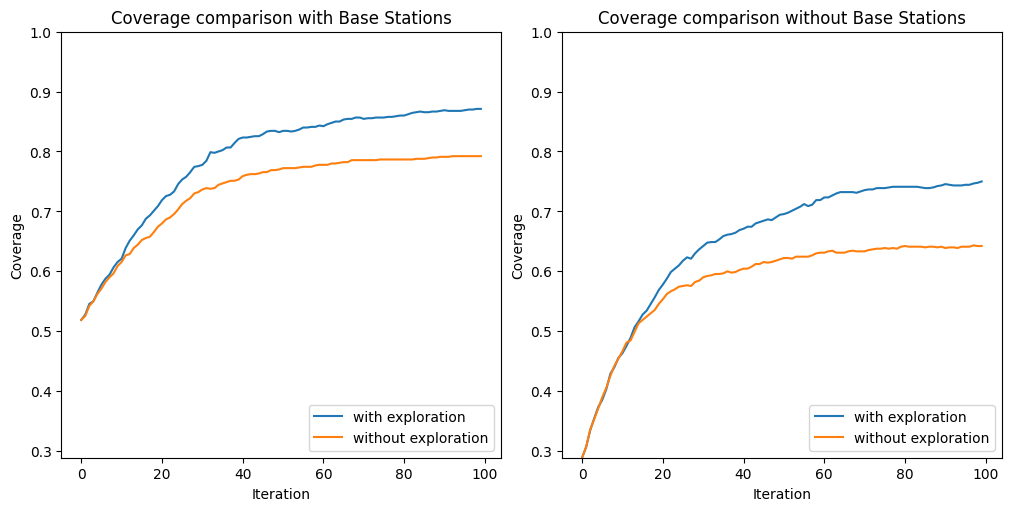
\includegraphics[width=1\textwidth]{img/ch4/experiment1/coverage_comparison.png}
    \caption[Grafici di copertura nel primo esperimento]{Confronto tra gli andamenti medi della copertura negli scenari di simulazione del primo esperimento.}
    \label{fig:confronto_cov_exp1}

    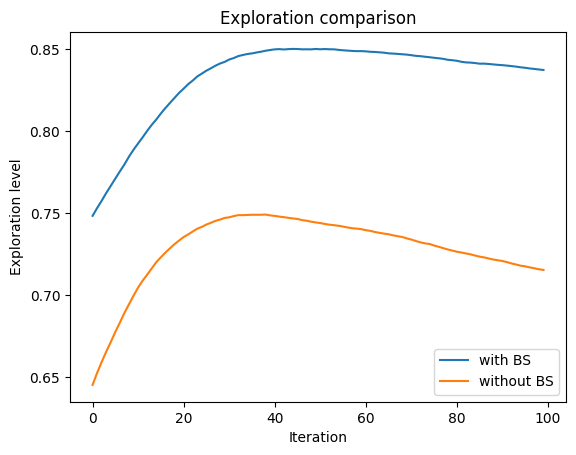
\includegraphics[width=0.5\textwidth]{img/ch4/experiment1/exploration_comparison.png}
    \caption[Grafici di esplorazione nel primo esperimento]{Confronto tra gli andamenti medi dell'esplorazione negli scenari di simulazione del primo esperimento.}
    \label{fig:confronto_expl_exp1}
\end{figure}

\begin{table}[t]
\centering
\begin{tabular}{|c|c|c|c|c|}
\hline
Simulazione & Massimo & Minimo & Media & Dev. standard \\
\hline
Con BS & 0.87 & 0.81 & 0.83 & 0.0129 \\
Senza BS & 0.76 & 0.67 & 0.71 & 0.0198 \\
\hline
\end{tabular}
\caption{\label{tab:exp1_expl_statistics}Primo esperimento, indici dei valori finali di esplorazione.}
\end{table}

\begin{figure}[p]
    \centering
    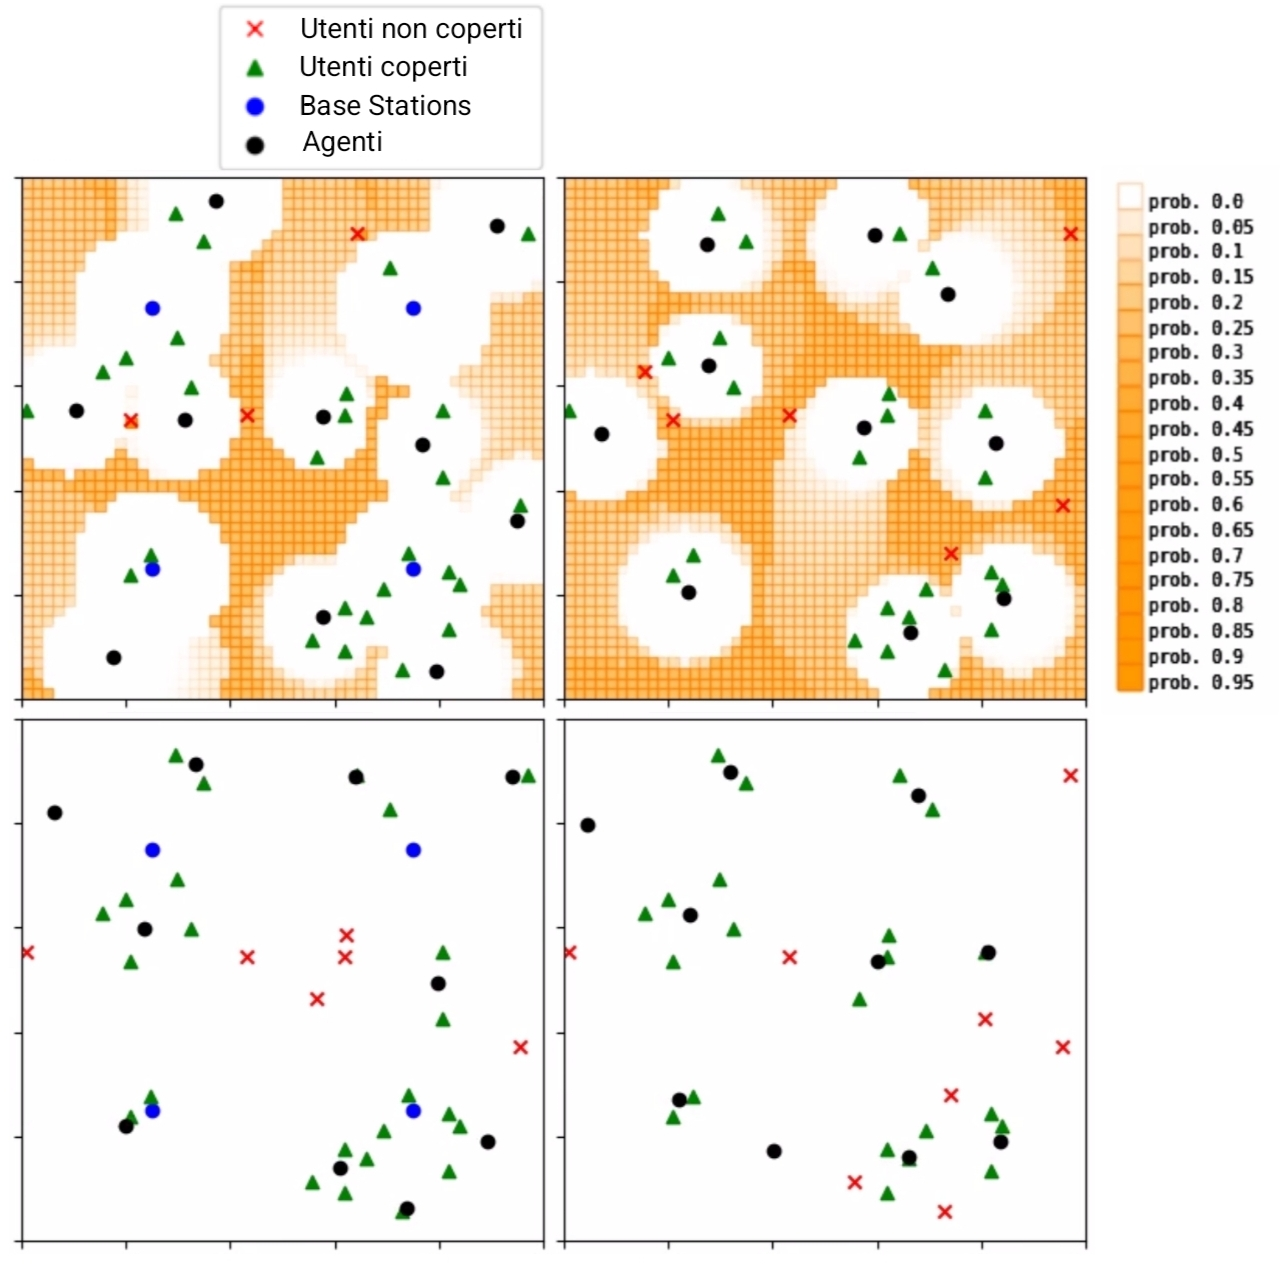
\includegraphics[width=1\linewidth]{img/ch4/experiment1/esempio_simulazioni.jpg}
    \caption[Simulazioni del primo esperimento]{Simulazioni del primo esperimento. In alto a sinistra, lo scenario con esplorazione e con BS; in alto a destra lo scenario con esplorazione ma senza BS; in basso gli scenari senza esplorazione.}
    \label{fig:esempio_simu_exp1}
\end{figure}
